\chapter{O equilíbrio químico: quociente e constante}\label{ch:g12:equilibrium}

Uma garrafa fechada de água com gás conserva o gás por meses; aberta,
ela fica choca numa tarde. Nada deu errado em nenhum dos dois casos. Na
garrafa fechada, o dióxido de carbono sai da água e volta para ela na
mesma velocidade, e a composição não muda; abra a tampa, e o gás que sai
não volta mais. Muitas reações se comportam assim: elas param antes que
algum \omterm{def:g7:chemical-reactions:reactant}{reagente} acabe, num balanço entre duas reações opostas. Este
capítulo descreve esse balanço com um único número.

\begin{recall}
O avanço $x$ de uma reação, o seu máximo $x_{\max}$ e as \omterm{def:g10:reaction-progress-table:limiting}{reações totais}
que o alcançam (\cref{ch:g10:reaction-progress-table}). As velocidades e
os \omterm{def:g12:reaction-rates:kinetic-factor}{fatores cinéticos} (\cref{ch:g12:reaction-rates}); um \omterm{def:g12:catalysis:catalyst}{catalisador} não
muda o \omterm{def:g10:reaction-progress-table:system}{estado final} (\cref{ch:g12:catalysis}).
\end{recall}

\begin{omfigure}
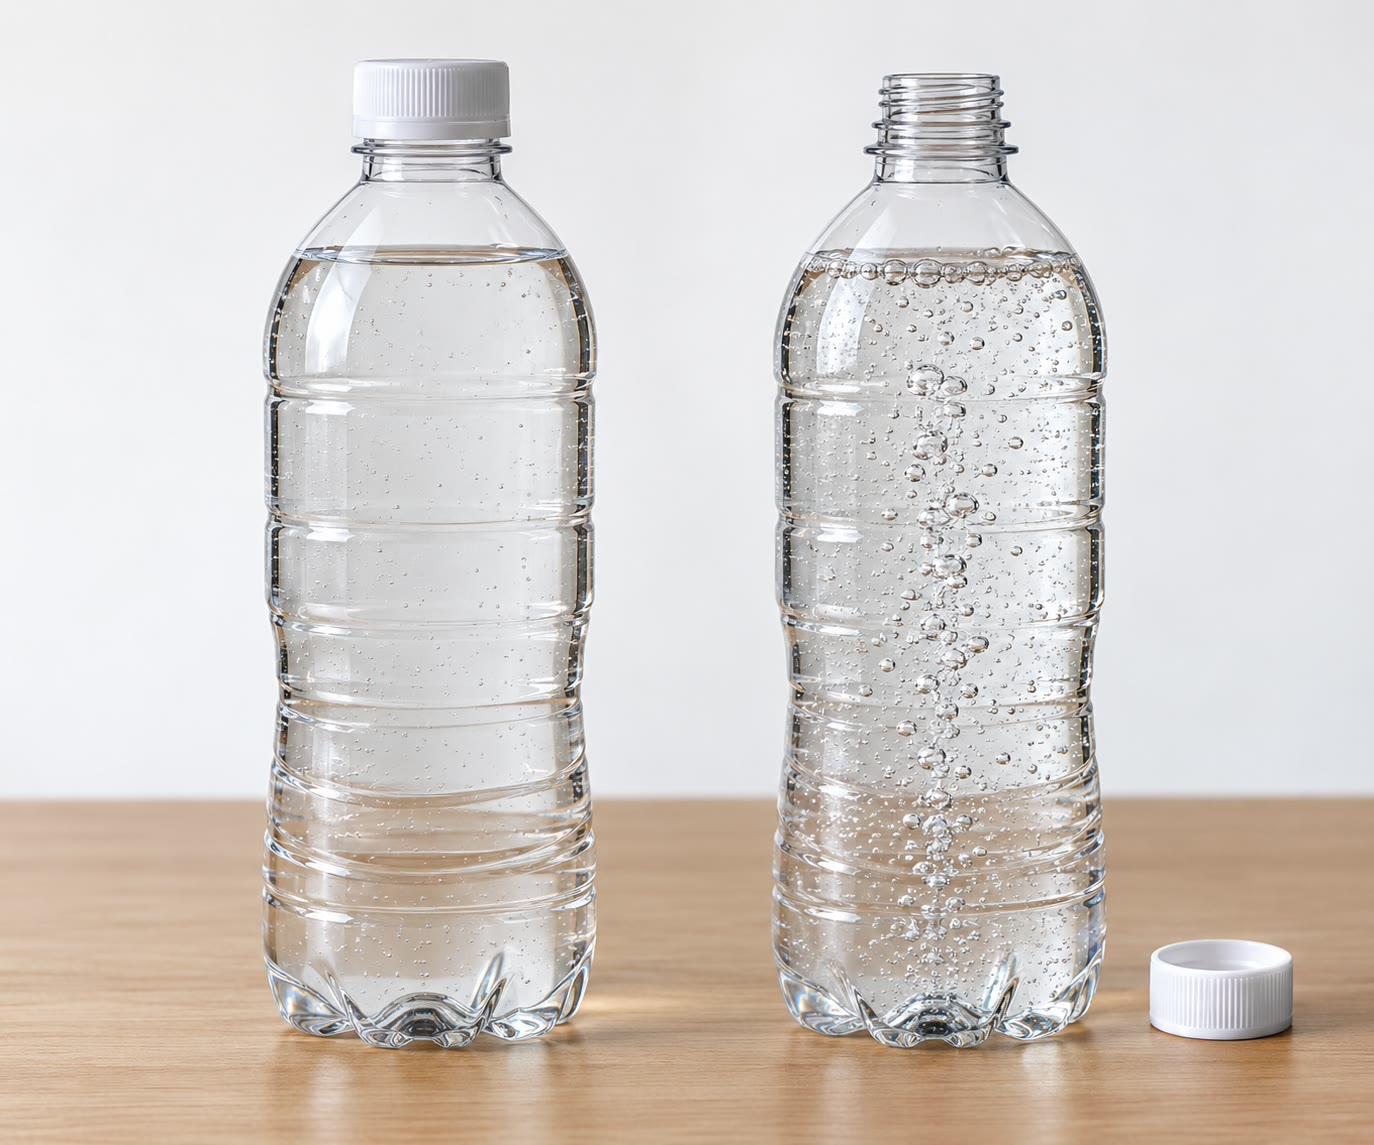
\includegraphics[width=0.45\linewidth,height=5cm,keepaspectratio]{images/book1/ai/g12-fizzy-bottles.jpg}

{\small Fechada, a água conserva o seu gás; aberta, o gás escapa e não
volta.}
\end{omfigure}

\section{As reações que não são totais}

\begin{definition}[Reação não total, taxa de avanço final]\label{def:g12:equilibrium:non-total}
Uma reação é uma \emph{reação não total}\index{reacao nao total@reação não total} se ela
para num avanço final $x_f$ menor que o seu \omterm{def:g10:reaction-progress-table:limiting}{avanço máximo} $x_{\max}$,
com todos os \omterm{def:g7:chemical-reactions:reactant}{reagentes} ainda presentes. A sua \emph{taxa de avanço
final}\index{taxa de avanco final@taxa de avanço final} é
\[
  \tau = \frac{x_f}{x_{\max}}, \qquad 0 < \tau < 1
\]
($\tau = 1$ para uma \omterm{def:g10:reaction-progress-table:limiting}{reação total}).
\end{definition}

\begin{example}[Um éster que para no meio do caminho]\label{ex:g12:equilibrium:berthelot}
% ledger: ester:berthelot
Aquecido com \qty{1}{mol} de etanol, \qty{1}{mol} de ácido etanoico
forma etanoato de etila e água,
\ce{CH3COOH + C2H5OH <=> CH3COOC2H5 + H2O}. A reação para quando cerca
de dois terços do ácido reagiram: $x_f = \qty{0.67}{mol}$ para
$x_{\max} = \qty{1}{mol}$, logo $\tau \approx 0.67$. Partindo de
\qty{1}{mol} de \omterm{def:g11:functional-groups:carboxylic-acid}{éster} e \qty{1}{mol} de água, a reação inversa também
para, com cerca de um terço do \omterm{def:g11:functional-groups:carboxylic-acid}{éster} hidrolisado: a mesma \omterm{def:g6:pure-substances-and-mixtures:mixture}{mistura} final.
\end{example}

\begin{history}[Berthelot e Péan de Saint-Gilles, 1862]
% ledger: ester:berthelot
Os químicos Marcellin Berthelot e Léon Péan de Saint-Gilles aqueceram
\omterm{def:g6:pure-substances-and-mixtures:mixture}{misturas} de ácido etanoico e etanol, e de etanoato de etila e água, por
longos períodos, e as analisaram. A partir de quantidades iguais de
ácido e de \omterm{def:g11:functional-groups:alcohol}{álcool}, a reação sempre parava em cerca de dois terços; a
partir de \omterm{def:g11:functional-groups:carboxylic-acid}{éster} e de água, em um terço de hidrólise; e eles notaram que
a quantidade de \omterm{def:g11:functional-groups:carboxylic-acid}{éster} formada a cada momento dependia do produto das
quantidades dos \omterm{def:g7:chemical-reactions:reactant}{reagentes}. O seu trabalho foi um dos primeiros estudos
quantitativos de um equilíbrio químico.
\end{history}

\section{O estado de equilíbrio}

\begin{definition}[Estado de equilíbrio]\label{def:g12:equilibrium:equilibrium-state}
Um sistema está num \emph{estado de equilíbrio}\index{estado de equilibrio@estado de equilíbrio}
quando a sua composição não muda mais, embora as reações direta e
inversa continuem acontecendo, na mesma velocidade. Uma reação que pode
chegar a esse estado é escrita com a seta dupla $\rightleftharpoons$.
\end{definition}

\begin{omfigure}
\begin{tikzpicture}
\begin{axis}[width=0.8\linewidth, height=6cm, xmin=0, xmax=200, ymin=0,
    ymax=1.05, xlabel={$t$ (\si{h})}, ylabel={quantidade de éster (\si{mol})},
    axis lines*=left, ymajorgrids, grid style={gray!20},
    tick label style={font=\small}, label style={font=\small},
    legend style={font=\small, at={(0.98,0.98)}, anchor=north east,
    draw=none, fill=white}, legend cell align=left]
  % ledger: ester:berthelot (K = 4; kinetics synthetic)
  \addplot[very thick, omDef] table[x=t, y=fromAcid] {figdata/out/grade-12-equilibrium.dat};
  \addplot[very thick, omProp] table[x=t, y=fromEster] {figdata/out/grade-12-equilibrium.dat};
  \addplot[dashed, black!60] coordinates {(0,0.6667) (200,0.6667)};
  \legend{a partir de 1 mol de ácido + 1 mol de álcool, a partir de 1 mol de éster + 1 mol de água}
  \node[font=\small, anchor=north east] at (axis cs:195,0.65) {equilíbrio: $\tfrac{2}{3}$ mol};
\end{axis}
\end{tikzpicture}

{\small A esterificação (em azul) e a hidrólise do \omterm{def:g11:functional-groups:carboxylic-acid}{éster} (em laranja)
chegam à mesma composição de equilíbrio, por lados opostos. (A escala de
tempo é um modelo; o valor final é o medido.)}
\end{omfigure}

\section{O quociente de reação}

\begin{notation}[Concentração padrão]\label{not:g12:equilibrium:c-standard}
$c^\circ = \qty{1}{mol/L}$ é a concentração padrão. Dividir uma
concentração por $c^\circ$ dá um número sem unidade com o mesmo valor:
$[\ce{A}]/c^\circ$.
\end{notation}

\begin{definition}[Quociente de reação]\label{def:g12:equilibrium:quotient}
Para uma reação em solução $a\,\ce{A} + b\,\ce{B} \rightleftharpoons c\,\ce{C} + d\,\ce{D}$, o \emph{quociente de
reação}\index{quociente de reacao@quociente de reação} num dado estado do sistema é
\[
  Q = \frac{\left([\ce{C}]/c^\circ\right)^c \left([\ce{D}]/c^\circ\right)^d}
           {\left([\ce{A}]/c^\circ\right)^a \left([\ce{B}]/c^\circ\right)^b} .
\]
Os sólidos, e o \omterm{def:g6:solutions-and-solubility:solute}{solvente} (a água numa \omterm{def:g6:solutions-and-solubility:solute}{solução aquosa}), não aparecem em
$Q$.
\end{definition}


\begin{example}[Escrever quocientes]\label{ex:g12:equilibrium:quotients}
Para \ce{CH3COOH + H2O <=> CH3COO- + H3O+} em água (o \omterm{def:g9:ions:ion}{íon} \ce{H3O+} é
apresentado no próximo capítulo), a água é o \omterm{def:g6:solutions-and-solubility:solute}{solvente}:
$Q = \dfrac{[\ce{CH3COO-}]\,[\ce{H3O+}]}{[\ce{CH3COOH}]\,c^\circ}$. Para a
dissolução de um sólido, \ce{AgCl(s) <=> Ag+ + Cl-}, o sólido fica de fora:
$Q = [\ce{Ag+}][\ce{Cl-}]/(c^\circ)^2$. Para a esterificação, em que as
quatro espécies estão na mesma \omterm{def:g6:pure-substances-and-mixtures:mixture}{mistura} líquida de volume $V$, os volumes
se cancelam e $Q = \dfrac{n_{\text{éster}}\, n_{\text{água}}}{n_{\text{ácido}}\, n_{\text{álcool}}}$.
\end{example}

\section{A constante de equilíbrio}

\begin{definition}[Constante de equilíbrio]\label{def:g12:equilibrium:constant}
O valor $Q_{eq}$ do \omterm{def:g12:equilibrium:quotient}{quociente de reação} no \omterm{def:g12:equilibrium:equilibrium-state}{estado de equilíbrio} é a
\emph{constante de equilíbrio}\index{constante de equilibrio@constante de equilíbrio} $K$ da
reação. Ela não tem unidade.
\end{definition}

\begin{proposition}[$K$ só depende da temperatura]\label{prop:g12:equilibrium:constant}
Para uma dada reação, $Q_{eq} = K$ em todo \omterm{def:g12:equilibrium:equilibrium-state}{estado de equilíbrio} a uma
dada temperatura, quaisquer que sejam as quantidades iniciais.
\end{proposition}

\begin{proof}
Admitido; isso é deduzido no volume do segundo ano da universidade. Isso
se verifica na esterificação: os dois experimentos da figura, iniciados
por lados opostos, dão o mesmo $Q_{eq}$.
\end{proof}

\begin{example}[O $K$ da esterificação]\label{ex:g12:equilibrium:k-ester}
% ledger: ester:berthelot
A partir de \qty{1}{mol} de ácido e \qty{1}{mol} de \omterm{def:g11:functional-groups:alcohol}{álcool}, o equilíbrio
contém $\frac{2}{3}$ \omterm{def:g10:the-mole:amount}{mol} de \omterm{def:g11:functional-groups:carboxylic-acid}{éster} e de água e $\frac{1}{3}$ \omterm{def:g10:the-mole:amount}{mol} de
ácido e de \omterm{def:g11:functional-groups:alcohol}{álcool}:
\[
  K = \frac{(2/3)\times(2/3)}{(1/3)\times(1/3)} = 4 .
\]
\end{example}

\begin{method}[O estado final de uma reação não total]\label{met:g12:equilibrium:final}
\begin{enumerate}
  \item Preencha a \omterm{def:g10:reaction-progress-table:extent}{tabela de avanço} com o avanço final desconhecido
        $x_f$.
  \item Escreva $Q_{eq}$ em função de $x_f$ e iguale-o a $K$.
  \item Resolva em $x_f$ (muitas vezes uma equação do segundo grau),
        conservando a raiz entre 0 e $x_{\max}$.
  \item Deduza as quantidades finais e $\tau = x_f/x_{\max}$.
\end{enumerate}
\end{method}

\begin{example}[Um excesso de álcool]\label{ex:g12:equilibrium:excess}
Com \qty{1}{mol} de ácido e \qty{2}{mol} de \omterm{def:g11:functional-groups:alcohol}{álcool}:
$\dfrac{x^2}{(1-x)(2-x)} = 4$, isto é, $3x^2 - 12x + 8 = 0$, cuja raiz
entre 0 e 1 é $x_f = \qty{0.845}{mol}$. Dobrar o \omterm{def:g11:functional-groups:alcohol}{álcool} aumenta o
\omterm{def:g10:synthesis-yield:yield}{rendimento}, contado sobre o ácido, de \qty{67}{\percent} para
\qty{85}{\percent}.
\end{example}

\section{Prever e deslocar a evolução}

\begin{proposition}[O sentido de evolução]\label{prop:g12:equilibrium:direction}
Se $Q < K$, o sistema evolui no sentido direto (os produtos aumentam)
até $Q = K$; se $Q > K$, ele evolui no sentido inverso; se $Q = K$, ele
está em equilíbrio e não muda.
\end{proposition}

\begin{proof}
Admitido: $Q$ aumenta quando a reação direta avança (os produtos do
numerador aumentam, os \omterm{def:g7:chemical-reactions:reactant}{reagentes} do denominador diminuem), e o sistema
se desloca para o estado em que $Q = K$.
\end{proof}

\begin{omfigure}
\begin{tikzpicture}[font=\small]
  \draw[->, thick] (0,0) -- (10,0) node[right] {$Q$};
  \draw[thick] (0,-0.12) -- (0,0.12) node[above] {0};
  \draw[very thick, omThm] (5,-0.25) -- (5,0.25) node[above] {$K$};
  \draw[->, very thick, omDef] (1.2,0.55) -- (4.4,0.55);
  \node[omDef, align=center] at (2.8,1.15) {$Q < K$: sentido direto};
  \draw[->, very thick, omProp] (8.8,0.55) -- (5.6,0.55);
  \node[omProp, align=center] at (7.2,1.15) {$Q > K$: sentido inverso};
  \node[align=center] at (5,-0.75) {$Q = K$: equilíbrio};
\end{tikzpicture}

{\small O quociente sempre se desloca em direção à constante.}
\end{omfigure}

\begin{remark}[Deslocar um equilíbrio]\label{rem:g12:equilibrium:shift}
Para obter mais produto de uma \omterm{def:g12:equilibrium:non-total}{reação não total}, pode-se acrescentar um
excesso de um \omterm{def:g7:chemical-reactions:reactant}{reagente} (o mais barato), ou retirar um produto à medida
que ele se forma: cada uma dessas ações torna de novo $Q < K$, e o
sistema avança. Retirar a água de uma esterificação (com um agente
secante, ou destilando-a) pode levar a reação quase até o fim. A garrafa
aberta de água com gás faz o mesmo com o dióxido de carbono que escapa.
\end{remark}

\begin{omfigure}
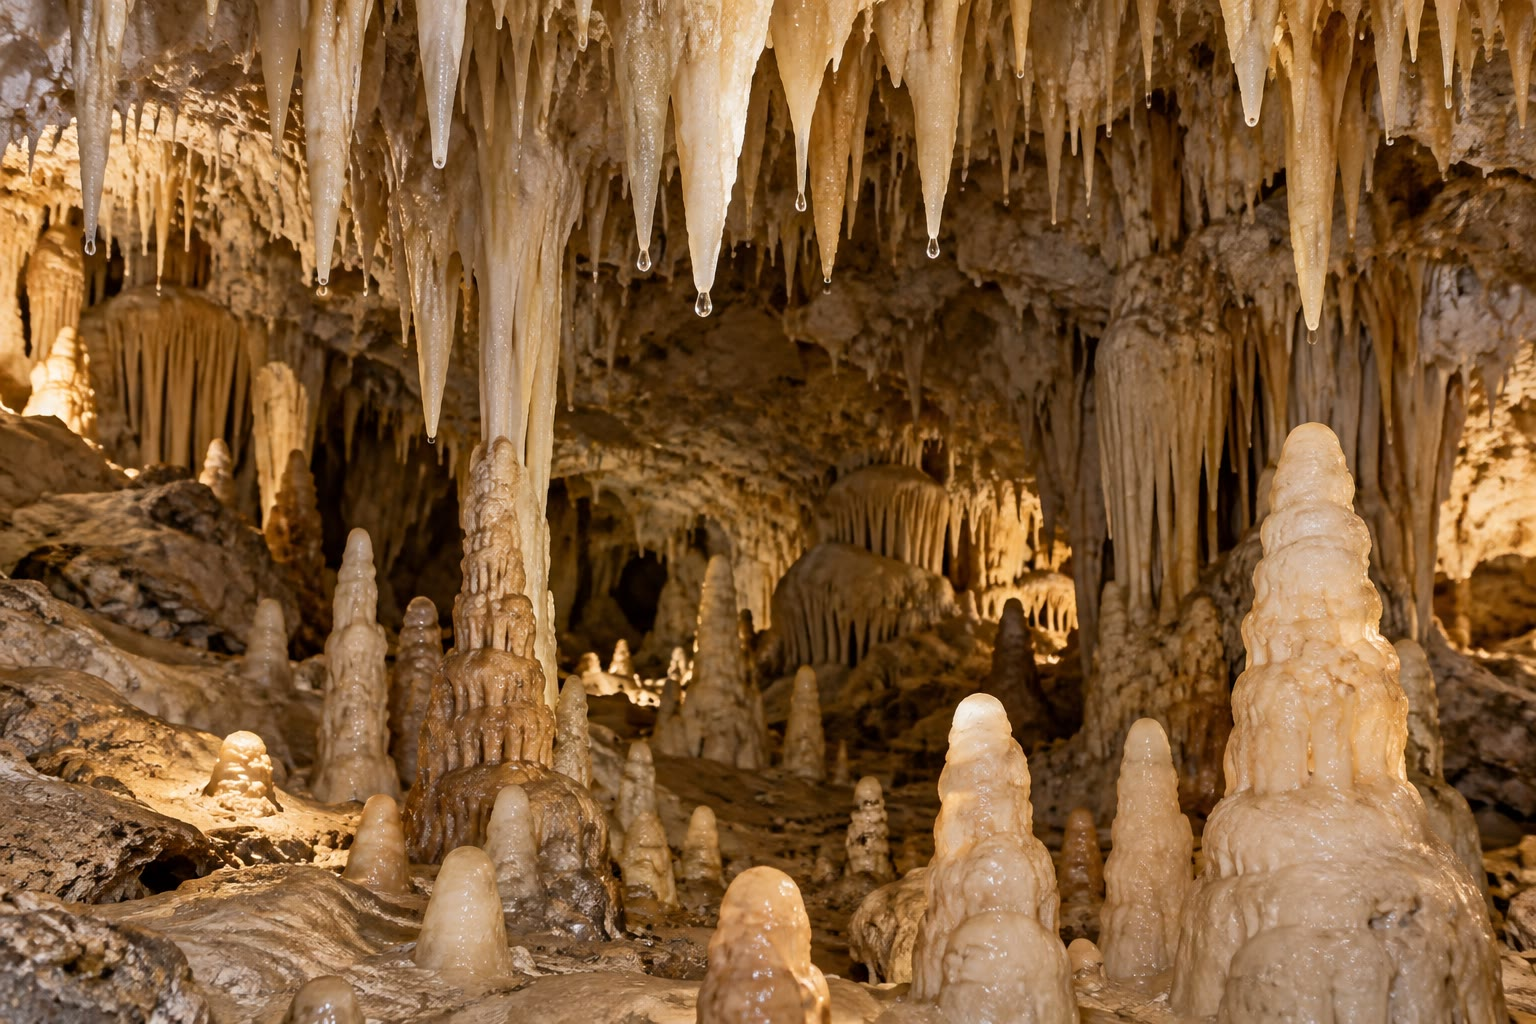
\includegraphics[width=0.45\linewidth]{images/book1/ai/g12-cave-stalactites.jpg}

{\small As estalactites crescem onde a água que pinga numa caverna perde
dióxido de carbono para o \omterm{def:g4:air-a-mixture-of-gases:air}{ar}: um equilíbrio do calcário dissolvido é
deslocado, e o carbonato de cálcio se deposita.}
\end{omfigure}

\section{Exercícios}

\begin{exercise}[$\star$]\label{exo:g12:equilibrium:1}
Escreva o \omterm{def:g12:equilibrium:quotient}{quociente de reação} de: (a) \ce{N2 + 3H2 <=> 2NH3} (gases, use
as concentrações); (b) \ce{CH3COOH + H2O <=> CH3COO- + H3O+} em água;
(c) \ce{CaCO3(s) <=> Ca^{2+} + CO3^{2-}}; (d) \ce{Fe^{3+} + SCN- <=>
FeSCN^{2+}}.
\end{exercise}

\begin{exercise}[$\star$]\label{exo:g12:equilibrium:2}
Uma reação tem $x_{\max} = \qty{0.050}{mol}$ e chega a
$x_f = \qty{0.020}{mol}$. Calcule $\tau$. A reação é total?
\end{exercise}

\begin{exercise}[$\star$]\label{exo:g12:equilibrium:3}
Para uma reação com $K = 10$, em que sentido evolui uma \omterm{def:g6:pure-substances-and-mixtures:mixture}{mistura} se
$Q = 2$? Se $Q = 50$? Se $Q = 10$?
\end{exercise}

\begin{exercise}[$\star$]\label{exo:g12:equilibrium:4}
Explique por que se diz que um equilíbrio é ``dinâmico''.
\end{exercise}

\begin{exercise}[$\star$]\label{exo:g12:equilibrium:5}
Um \omterm{def:g12:catalysis:catalyst}{catalisador} muda $K$? E o tempo necessário para chegar ao equilíbrio?
Explique.
\end{exercise}

\begin{exercise}[$\star\star$]\label{exo:g12:equilibrium:6}
Misturam-se \qty{2.0}{mol} de ácido etanoico e \qty{2.0}{mol} de etanol
($K = 4$). Calcule as quantidades finais das quatro espécies.
\end{exercise}

\begin{exercise}[$\star\star$]\label{exo:g12:equilibrium:7}
Uma \omterm{def:g6:pure-substances-and-mixtures:mixture}{mistura} contém \qty{0.5}{mol} de cada um: ácido etanoico, etanol,
etanoato de etila e água. Calcule $Q$. Em que sentido ela evolui?
\end{exercise}

\begin{exercise}[$\star\star$]\label{exo:g12:equilibrium:8}
Usando a figura dos dois experimentos, leia a quantidade de \omterm{def:g11:functional-groups:carboxylic-acid}{éster} depois
de \qty{20}{h} em cada experimento. A partir de quando se pode
considerar que o sistema está em equilíbrio?
\end{exercise}

\begin{exercise}[$\star\star$]\label{exo:g12:equilibrium:9}
Partindo de \qty{1}{mol} de \omterm{def:g11:functional-groups:carboxylic-acid}{éster} e \qty{1}{mol} de água ($K = 4$ para
a esterificação, logo $1/4$ para a hidrólise), calcule as quantidades
finais pelo método do capítulo, e compare com o experimento de
esterificação.
\end{exercise}

\begin{exercise}[$\star\star$]\label{exo:g12:equilibrium:10}
Por que o sólido não aparece no quociente de
\ce{AgCl(s) <=> Ag+ + Cl-}? Acrescentar mais sólido desloca o
equilíbrio?
\end{exercise}

\begin{exercise}[$\star\star$]\label{exo:g12:equilibrium:11}
Numa garrafa fechada de água com gás, o dióxido de carbono sai da água e
entra nela na mesma velocidade. Escreva o equilíbrio
\ce{CO2(aq) <=> CO2(g)} e explique, com $Q$ e $K$, por que a água fica
choca quando a garrafa é aberta.
\end{exercise}

\begin{exercise}[$\star\star\star$]\label{exo:g12:equilibrium:12}
Uma esterificação de \qty{1}{mol} de ácido e \qty{1}{mol} de \omterm{def:g11:functional-groups:alcohol}{álcool}
chega ao equilíbrio. Retira-se então a metade da água presente. Calcule
o novo $Q$, diga em que sentido o sistema evolui e encontre a nova
quantidade final de \omterm{def:g11:functional-groups:carboxylic-acid}{éster}.
\end{exercise}

\begin{exercise}[$\star\star\star$]\label{exo:g12:equilibrium:13}
Mostre que a constante da reação inversa é $1/K$. Qual é a constante da
hidrólise do etanoato de etila?
\end{exercise}

\begin{exercise}[$\star\star\star$]\label{exo:g12:equilibrium:14}
Um químico \omterm{def:g6:pure-substances-and-mixtures:mixture}{mistura} \qty{1}{mol} de ácido, \qty{1}{mol} de \omterm{def:g11:functional-groups:alcohol}{álcool},
\qty{2}{mol} de \omterm{def:g11:functional-groups:carboxylic-acid}{éster} e \qty{0.5}{mol} de água. Vai acontecer alguma
coisa? Explique.
\end{exercise}

\begin{exercise}[$\star\star\star$]\label{exo:g12:equilibrium:15}
Que excesso de \omterm{def:g11:functional-groups:alcohol}{álcool} (quantidade por \omterm{def:g10:the-mole:amount}{mol} de ácido) é necessário para
esterificar \qty{95}{\percent} do ácido? Resolva $\dfrac{0.95^2}{0.05(n - 0.95)} =
4$.
\end{exercise}

\section{Problema: o éster de Berthelot}

\begin{problem}[{Problema de fim de semana --- quanto éster quando o álcool
é posto em excesso triplo?}]
\label{pb:g12:equilibrium:1}
% ledger: ester:berthelot, aw:C, aw:H, aw:O
O etanoato de etila, um \omterm{def:g6:solutions-and-solubility:solute}{solvente} e um aromatizante, é fabricado a partir
do ácido etanoico e do etanol. Em 1862, Berthelot e Péan de Saint-Gilles
descobriram que, a partir de quantidades iguais de ácido e de \omterm{def:g11:functional-groups:alcohol}{álcool}, a
reação para quando cerca de dois terços do ácido reagiram.

\medskip
\noindent\textbf{Parte I --- A reação.}
\begin{enumerate}
  \item Escreva a equação da esterificação, com \omterm{def:g11:organic-skeletons:formulas}{fórmulas estruturais
        condensadas}.
  \item Por que ela é escrita com uma seta dupla?
  \item Escreva o seu \omterm{def:g12:equilibrium:quotient}{quociente de reação} em \omterm{def:g10:the-mole:amount}{quantidades de matéria}.
  \item A partir de \qty{1}{mol} de ácido e \qty{1}{mol} de \omterm{def:g11:functional-groups:alcohol}{álcool}, qual
        é $x_{\max}$? Qual é $x_f$, segundo o resultado de Berthelot?
  \item Calcule $\tau$.
\end{enumerate}

\medskip
\noindent\textbf{Parte II --- A constante.}
\begin{enumerate}[resume]
  \item Dê as quantidades finais das quatro espécies.
  \item Calcule $K$.
  \item Partindo de \qty{1}{mol} de \omterm{def:g11:functional-groups:carboxylic-acid}{éster} e \qty{1}{mol} de água,
        Berthelot encontrou um terço hidrolisado. Mostre que isso está
        de acordo com o mesmo $K$.
  \item Por que $K$ tem de ser o mesmo nos dois casos?
\end{enumerate}

\medskip
\noindent\textbf{Parte III --- Um excesso triplo de \omterm{def:g11:functional-groups:alcohol}{álcool}.}
\begin{enumerate}[resume]
  \item A partir de \qty{1}{mol} de ácido e \qty{3}{mol} de \omterm{def:g11:functional-groups:alcohol}{álcool},
        preencha a \omterm{def:g10:reaction-progress-table:extent}{tabela de avanço}.
  \item Escreva a equação $Q_{eq} = K$ e mostre que ela se torna
        $3x^2 - 16x + 12 = 0$.
  \item Resolva-a, e conserve a raiz que tem sentido.
  \item Que fração do ácido é esterificada?
  \item Calcule a massa de \omterm{def:g11:functional-groups:carboxylic-acid}{éster} obtida.
\end{enumerate}

\medskip
\noindent\textbf{Parte IV --- Retirar a água.}
\begin{enumerate}[resume]
  \item A partir do equilíbrio equimolar, a água é retirada à medida que
        se forma. Explique com $Q$ por que a reação continua.
  \item Se toda a água pudesse ser retirada, qual seria o \omterm{def:g10:synthesis-yield:yield}{rendimento}?
  \item Por que, em geral, é o \omterm{def:g11:functional-groups:alcohol}{álcool}, e não o ácido, que se põe em
        excesso? (Pense no custo e na separação dos produtos.)
  \item Aquecer a \omterm{def:g6:pure-substances-and-mixtures:mixture}{mistura} muda o \omterm{def:g10:reaction-progress-table:system}{estado final}, ou só o tempo para
        alcançá-lo? (A esterificação quase não libera calor.)
  \item Dê a resposta final: que fração do ácido é esterificada com um
        excesso triplo de \omterm{def:g11:functional-groups:alcohol}{álcool}?
\end{enumerate}
\end{problem}
